%!TEX root = spack-sc15.tex

\subsection{Concretization}
\label{sec:concretization}

We have discussed Spack's internal software DAG model, and we have shown
how the spec syntax can be used to quickly specify a partially constrained
software DAG.  We say such a DAG is {\it abstract}, as it could potentially
describe more than one software configuration. Before Spack builds a spec, it
must ensure the following conditions:
\begin{enumerate}
\item No package in the spec DAG is missing dependencies.
\item No package in the spec DAG is virtual.
\item All parameters are set for all packages in the DAG.
\end{enumerate}
If a spec meets all of these criteria, we say it is {\it concrete}.
{\it Concretization} is the central component of Spack's build
process that allows it to reduce an unconstrained abstract
description to a concrete build.

Spack's concretization algorithm is shown in Figure~\ref{fig:concretization}.
The process starts when a user invokes {\tt spack install} and requests that a
spec be built.  Spack converts the spec to an abstract DAG.
It then builds a {\it separate} spec DAG for any constraints encoded
by directives in package files.
%
Spack intersects the constraints of the two DAGs package by package, and it
checks each parameter for inconsistencies.  Inconsistencies can arise if, for example,
the user inadvertently requests two versions of the same package, or if a
package file depends on a different version than the user requested.
Likewise, if the package and the user specified different compilers, variants,
or platforms for particular packages, Spack will stop and notify
the user of the conflict. If the user or package specifies version ranges,
they are intersected, and if the ranges do not overlap, an error is raised.
When the intersection succeeds, Spack has a single DAG with the merged
constraints of the user and the package files.

The next part of the process is iterative.
If any node is a virtual dependency, Spack replaces it with with a
suitable interface provider.  It does this by building a reverse
index from virtual packages to providers using the {\tt provides when}
directives (Section~\ref{sec:virtual}). If multiple providers
satisfy the virtual spec's constraints,
Spack consults site and user policies to select the ``best'' possible
provider.  The selected provider may {\it itself} have virtual dependencies,
this process is repeated until there are no more virtual packages in the DAG.

With the now non-virtual DAG, Spack again consults site and user preferences for
variants, compilers, and versions to resolve any remaining abstract nodes.
Adding a variant like {\tt +mpi} may cause a package to depend on more
libraries (as in Section~\ref{sec:constraints}). The concretization algorithm
evaluates conditions from {\tt when} clauses on the DAG, and if there are
new libraries or other changes, the cycle begins again.
Spack currently avoids an exhaustive search by using a greedy algorithm.
It will not backtrack to try other options if its first policy choice leads
to an inconsistency.  Rather, it will raise an error and the user must resolve
the issue by being more explicit.  The user might toggle a variant, or she might
force the build to use a {\it particular} MPI implementation
by supplying \verb|^openmpi| or \verb|^mpich|.  We leave automatic constraint
space exploration for future work.


\begin{figure}
	\centering
	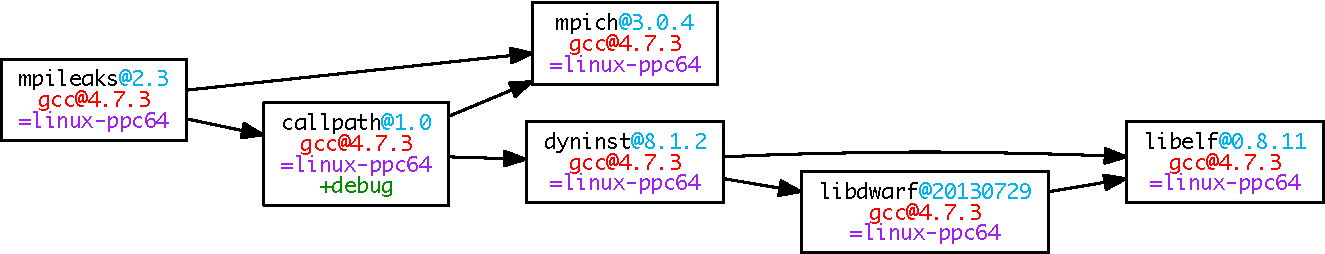
\includegraphics[width=\columnwidth]{specs/mpileaks-concrete.pdf}
	\caption{
		Concretized spec from Figure~\ref{fig:specs-mpileaks}.
		\label{fig:specs-mpileaks-concrete}
	}
\end{figure}
On completion, the concretization outputs a fully concrete spec DAG.
Figure~\ref{fig:specs-mpileaks-concrete} shows a concrete DAG with architectures,
compilers, versions, variants, and all dependencies resolved.
This fulfills Spack's guarantees.
%
At install time, Spack constructs a package object for each node in the spec DAG
and traverses the DAG in a bottom-up fashion.  At each node, it invokes the package's
{\tt install} method.  For the {\tt spec} parameter to {\tt install}, it passes
a sub-DAG rooted at current node (also a concrete spec).  Package authors must
query the spec in {\tt install} to handle different configurations.

\subsubsection{Concretization Runtime}
\label{sec:concretization-overhead}

\begin{figure}
	\centering
	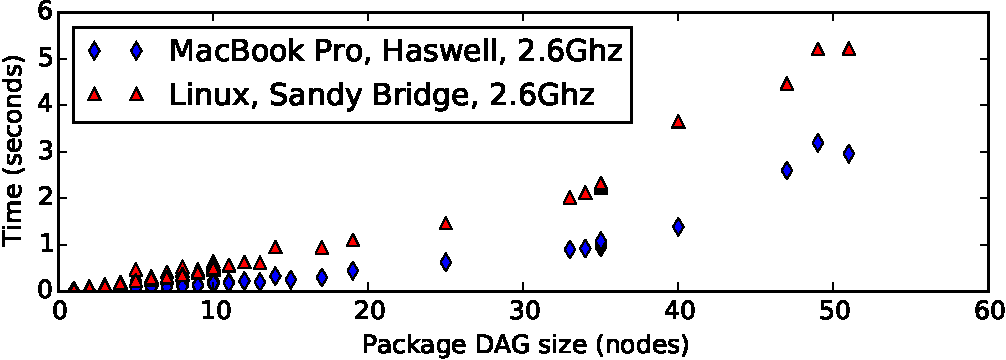
\includegraphics[width=.95\columnwidth]{figs/concretization-overhead/concretization-times.pdf}
	\caption{
		Concretization running time for 245 packages.
		\label{fig:concretization-time}
	}
\end{figure}

Figure~\ref{fig:concretization-time} shows the running time of concretization vs.
package DAG size in nodes.  We generated this plot by running {\tt concretize}
on all of Spack's 245 packages. We tested on three LLNL cluster front-end nodes:
a 2.3GHz Intel Haswell node and a 2.6 GHz Intel Sandy Bridge node on our Linux
clusters, and the 3.6 GHz IBM Power7 front-end node of a Blue Gene/Q system.
Each point is the average of 10 trials.  For all but the 10
largest packages, concretization takes less than 2 seconds on all machines.
For larger DAGs, we begin to see a quadratic trend, but even for 50 nodes or more, 
concretization takes less than 4 seconds on the Haswell machine and 9 seconds on the 
Power7.
%
We expect this performance from our greedy, fixed-point method, and
it is sufficient for the packages we have built so far.
Its running time is insignificant compared to the build time of
most packages, and it only executes
once per build. 
More generally, concretization is an instance of the constraint
satisfaction problem, which is NP-complete. While concretization could become
more costly, we do not expect to see packages with
thousands of dependencies in the near future. We do not expect
it to become a bottleneck, even if we use a full constraint solver.

\subsubsection{Shared sub-DAGs}
\label{sec:directory-layout}

We mentioned in Section~\ref{sec:packages} that each unique configuration is
guaranteed a unique install prefix. Spack uses the concrete {\it spec}
to generate a unique path, shown in Table~\ref{tab:naming-conventions}.
To prevent the directory name from growing too long, Spack uses a SHA hash of
dependencies' specs as the last directory component.  This
does {\it not} mean that Spack rebuilds every library for each new configuration.
If two configurations share a sub-DAG, then the sub-DAG's configuration will
be reused.  Figure~\ref{fig:reuse} shows how the {\tt dyninst} sub-DAG is used for
both the {\tt mpich} and {\tt openmpi} builds of {\tt mpileaks}.


\subsubsection{Reproducibility}


For reproducibility, and to preserve provenance, Spack stores a number of
files in the installation directory that document how the installed package was
built.  These include the {\tt package.py} file used to build, a build log
containing output and error messages, and a file containing the complete
concrete spec for the package {\it and} its dependencies. The spec file can be
used later to reproduce the build, even if concretization preferences have changed.

\subsubsection{Site policies and build complexity}

Our experience with manual installs helped us understand that much of the complexity
of building HPC software comes from the size of the build parameter space.
As mentioned, there are only a few parameters that typical users care about.
The rest add unneeded complexity.  When building manually, LLNL staff
tend to make arbitrary choices about the secondary build parameters,
or they add logic to build scripts to make these choices.
Manually built software is generally not installed in a consistent manner.

Concretization provides two benefits.  First, it allows users and staff to
request builds with a minimal spec expression, while still providing a
mechanism for the site and the user to make consistent, repeatable choices about
other build parameters.  For example, the site or the user can set default versions
to use for any library that is not specified explicitly.
%
Second, concretization reduces the burden of packaging software, because
package authors do not have to make these decisions.  There is no
need for packages to contain complicated checks, or for packages to be overly
specific about versions.  Other multi-configuration systems like Nix, EasyBuild,
and HashDist require the package author to write a mostly concrete build spec in advance.
We believe that this puts undue burden on the package author, and it makes the task
of changing site policies within a software stack difficult.  Spack
separates these concerns.

\begin{figure}\centering
   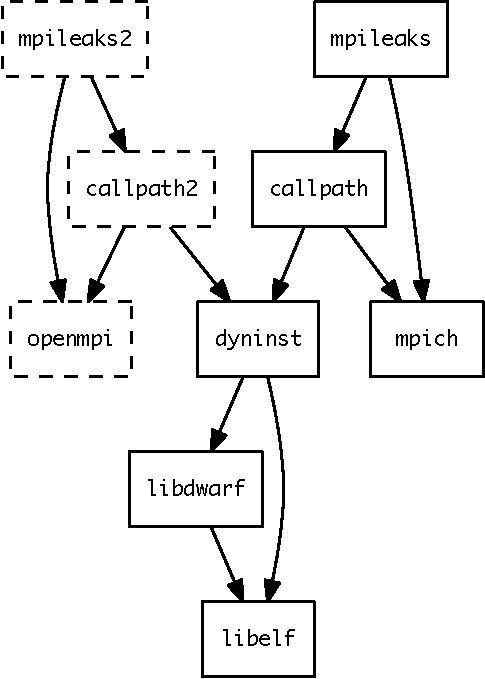
\includegraphics[width=.9\linewidth]{specs/rpaths.pdf}
   \caption{
       {\tt mpileaks} built with {\tt mpich}, then {\tt openmpi}.
       \label{fig:reuse}
   }
\end{figure}

